
\begin{frame}[t]{Recap}

\framesubtitle{Starfish: a quick recap}

\begin{itemize}
  \item System to improve knowledge sharing
  \item Network of linked (directed) documents
  \item Goal: create system that can automaticaly propose new links
\end{itemize}


\end{frame}




\begin{frame}[t]{Progress}

  \huge{Sprint One or Week Two}

\end{frame}




\begin{frame}[t]{Progress}

\framesubtitle{What did we set out to do?}

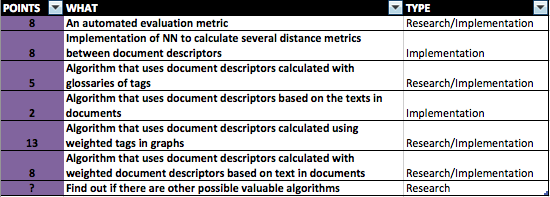
\includegraphics[width=8cm]{sprintt}

\end{frame}

\begin{frame}[t]{Progress}

\framesubtitle{What did we do?}

\begin{itemize}
\item Software skeleton
\item Nearest Neighbor
\item Different vector distance metrics
\item Document vectorizers \\
  \begin{itemize}
    \item (Weighted) tag glossary descriptor
    \item Text descriptor
    \item Tag descriptor
    \item Smoothed tag descriptor
  \end{itemize}
\item Research on other methods
\end{itemize}

\end{frame}



\begin{frame}[t]{Progress}

\framesubtitle{What didn't we do?}

\begin{itemize}
\item Automated evaluation metric
\end{itemize}

\end{frame}



\begin{frame}[t]{Progress}

\framesubtitle{Deliverable}

A program that can given a network and a new document propose new
links between the new and known documents.

\addvspace{3mm}
{\tt \$ documentlinker\\ Usage: -vectorizer <algorithm> -distance <cosine/eucledian>}

\pause
\addvspace{3mm}
Does not accept a new document yet, but will propose new documents for every
document in the data set.

\end{frame}
